\subsection*{research}
i discovered \autocite{rf-amp-classics} (see \localfile{../research/books/}),
an \arrl book on \rf amplifiers, and skimmed through it. some items of
interest:
\begin{enumerate}
	\item \autocite[p.~1 dash 41]{rf-amp-classics}: class-E power
	amplifiers are a highly power- and parts-efficient amplifier topology,
	utilizing a single active element and a tuned load. the article,
	``High-Efficiency Class-E Power Amplifiers,'' claims 21-fold power
	improvement over class-A for a given dissipated power. since our
	fractional bandwidth is not that high (\textasciitilde 2.5 \%), we
	could get away with a Q of 40 in the tuned load and still transmit
	across the band, so class-E might be feasible! the circuit used in the
	article is reproduced in figure \ref{fig:class-e-from-article}.

	\begin{figure}[H]
		\centering
		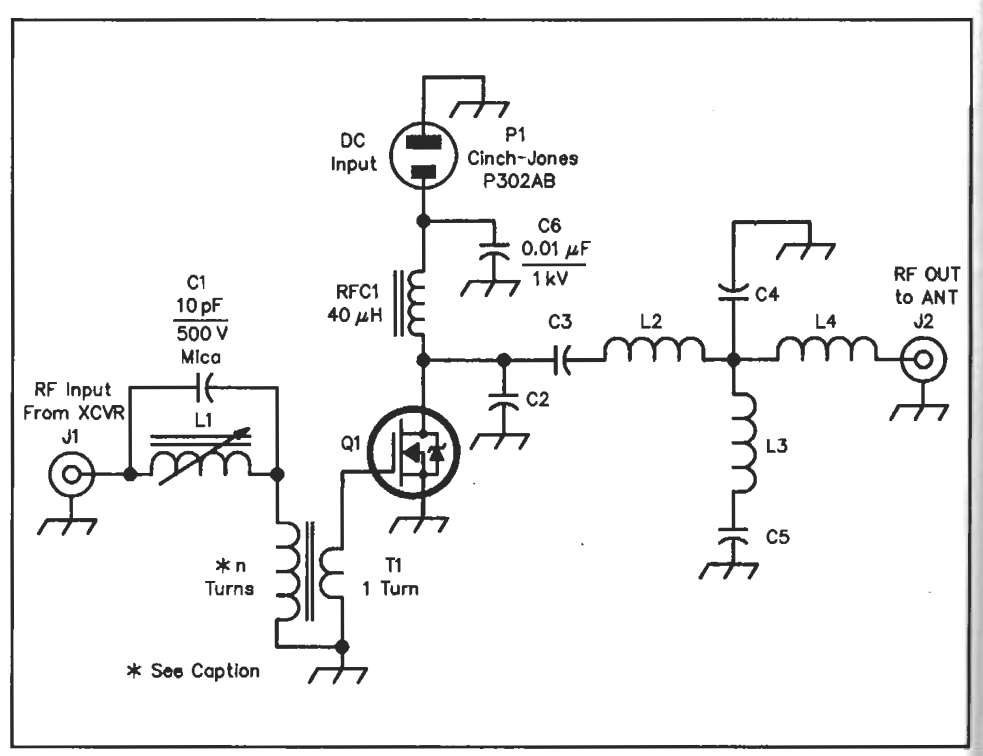
\includegraphics[width=.7\textwidth]{class-e-from-article.png}
		\caption{a class-E amplifier.}
		\label{fig:class-e-from-article}
	\end{figure}
\end{enumerate}

\subsection*{code}
i typeset this log and wrote the first two entries.
